\section{Discussion}
\label{sec:discussion}

\subsection{Principal findings}

Three findings follow from Section~\ref{sec:results}, each obtained against attacks that
were synthesised as waveforms and tracked through the receiver.

Clean detection performance does not predict resistance to transmitted attack. The random
forest attains both the highest clean $F_1$ score and the lowest false alarm rate of the
fourteen detectors, and it is nonetheless evaded by 43.7 percent of the transmitted
takeover attacks, with an exact interval of [0.348, 0.528]. The effect is not confined to
one model: the four detectors with the highest clean $F_1$ are evaded on 0.226 of their
detector-attack pairs against 0.106 for the remaining ten, a difference significant at
$p = 2.8 \times 10^{-10}$. Because all fourteen detectors are read at the same recall
floor, this cannot be attributed to differences in threshold placement, and because the
attacks were selected without reference to any detector, it cannot be attributed to
adversarial optimisation against a particular model.

The relationship is a contrast between groups and not a monotone trend across
architectures. Section~\ref{sec:res_stats} reports a Spearman correlation of $+0.41$
between clean $F_1$ and evaded fraction which is not significant at $n = 14$, because the
support vector machine combines the worst clean score with the second highest evasion
count. Both results are reported, and the contrast is the one the
evidence supports.

Where resistance does appear, it is purchased with false alarms. Five detectors flag every
one of the 126 attacks, and those same five flag between 46 and 74 percent of authentic
samples. A receiver alarming on half of its authentic observations would be
disabled in service, so this resistance is not operationally available, and the pattern is
the accuracy against robustness trade of Section~\ref{sec:rw_adversarial} appearing in a
GNSS setting. Figure~\ref{fig:tradeoff} shows the same point across the full set of
criteria a deployment decision weighs: no detector dominates on all of them, and the
orderings induced by different criteria disagree, so no single scalar ranks the set.

% Figure source: figures_src/fig_legacy.py
\begin{figure}[t]
\centering
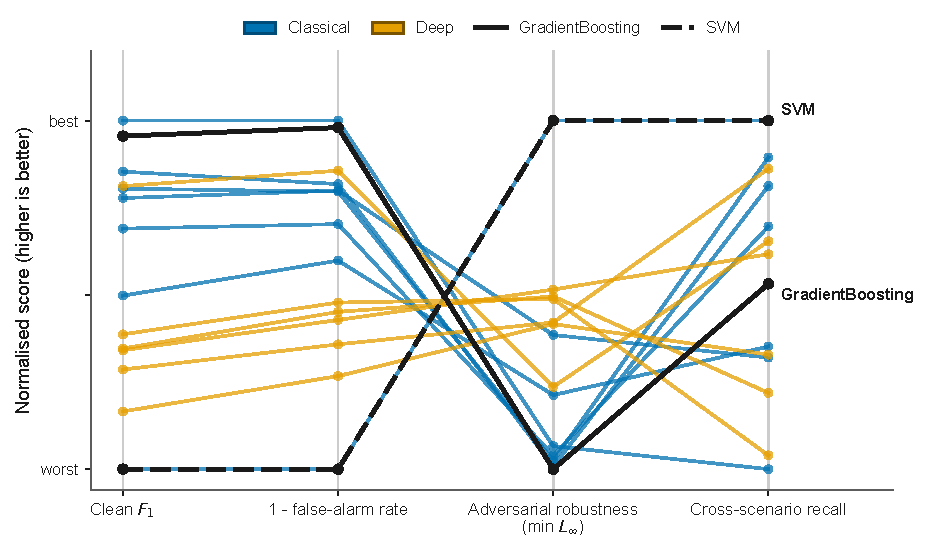
\includegraphics[width=\linewidth]{figures/fig11_tradeoff_parallel.pdf}
\caption{Every detector across the criteria a deployment decision would weigh, each normalised so higher is better. No detector is best on all of them, and the orderings disagree, so a single accuracy figure cannot rank them.}
\label{fig:tradeoff}
\end{figure}

A missed detection is consequential and not benign. The attack propagated through the
navigation stage drove the receiver clock at the rate the transmitter was configured to
impose, to within 0.05 percent, while the detector with the best clean performance
classified 98.8 percent of its samples as authentic. Detection failure and navigation
domain effect were measured on the same attack and the same recording, so the two are not
independent observations juxtaposed after the fact.

\subsection{Implications for detector evaluation}

Evaluating at the waveform level fixes the interpretation of the resulting failure rates.
A displacement applied directly to a table of receiver observables corresponds to an attack
only if some incident waveform produces that displacement. Several observables a receiver
reports are computed from the same correlator accumulations and cannot be varied
independently, so an evaluation that varies them independently may report vulnerability to
a receiver state that no transmission realises. When the attack is generated as a signal,
the observables are by construction whatever the receiver computed while tracking it, and
every constraint receiver processing imposes is satisfied because that processing imposed
it.

Section~\ref{sec:res_compare} quantifies what this changes. For the tree based detectors
the feature space and waveform level evaluations agree, and the fragility those models
exhibit is a property of the models and not of either evaluation. For the support
vector machine the two disagree entirely: its minimum perturbation is the largest in the
study, which taken alone would identify it as the most robust detector, yet it is evaded by
53 of the 126 transmitted attacks. Its false alarm rate of 0.960 reconciles the two
readings, since a classifier that flags almost everything is expensive to cross in feature
space while remaining useless as a monitor. The conclusion is not that one evaluation is
invalid, but that a perturbation magnitude reported without the false alarm rate that
accompanies it can invert the ordering it appears to establish.

A related limitation of accuracy based evaluation appears under distribution shift.
Figure~\ref{fig:generalization} reports recall on data withheld from training, holding out
either an entire attack scenario or individual satellites. Recall falls in both cases,
which indicates that the detectors depend on conditions present in their training data even
before an adversary is introduced.

% Figure source: figures_src/fig_legacy.py
\begin{figure*}[t]
\centering
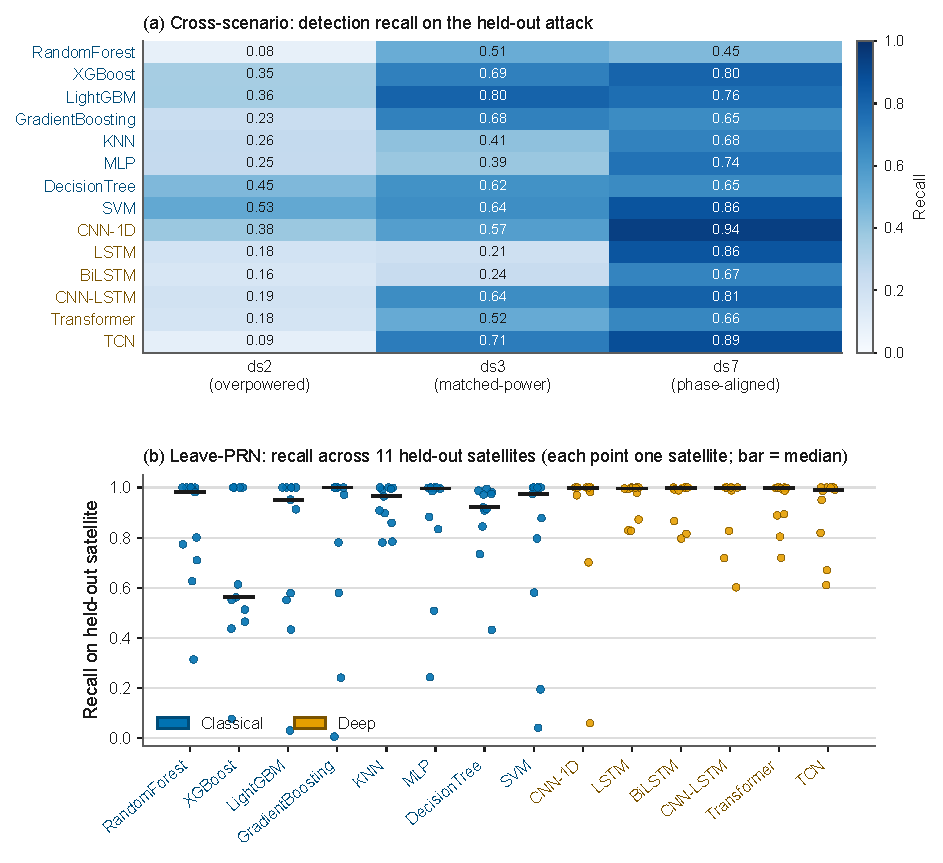
\includegraphics[width=\textwidth]{figures/fig08_generalization.pdf}
\caption{Detection recall on data held out from training. Panel (a) holds out a whole attack scenario and panel (b) holds out satellites one at a time. Recall falls in both, so the detectors depend on conditions present in their training data.}
\label{fig:generalization}
\end{figure*}

\subsection{Implications for receiver integrity}

The transmitter settings evaluated here were selected without reference to any detector,
and 126 of them capture a receiver. Approximately two fifths of those evade the strongest
detector tested, and none of that required knowledge of the detector, access to its
gradients, or the ability to query it. An adversary possessing any of those capabilities
would be strictly stronger.

For a receiver integrity monitor the practical consequence is that detection quality
measured on a fixed corpus is not a security property. It characterises behaviour on that
corpus, and a detector intended to resist an adversary must be characterised against
signals the adversary can select and emit, with the false alarm rate reported alongside.

The false alarm rates observed here carry a further implication independent of any
adversary. At a recall floor of 0.95 they span 0.337 to 0.960, so no detector in this study
is usable as a standalone single epoch integrity monitor even in the absence of an attacker.
A deployed monitor would necessarily combine decisions across epochs and across satellites,
trading detection latency against alarm rate, and the per epoch quantities reported here
are the inputs to such a scheme and not a substitute for it.

\subsection{Scope and limitations}

The adversary is restricted in the four respects set out in Section~\ref{sec:threat}, and
each restriction reduces its capability, so the failure rates reported are a lower bound on
what an unrestricted adversary could achieve. The power condition illustrates the point.
Requiring the counterfeit to exceed the authentic signal follows the established account
of capture, and it is one of the two conditions, with the code being dragged, that select
126 of the 209 swept settings as operative. Capture at lower power has since been reported by other means
\citep{liu2026dimas}, which would enlarge the operative subset and so enlarge the set of
transmissions a detector must withstand. Relaxing the condition could therefore only
raise the counts reported here.

The study covers one signal, GPS L1 C/A, and one stationary receiver at a surveyed
location. Whether the same detectors behave equivalently on other civil signals, or on a
moving platform whose dynamics enter the observables, is not established here. The
generator itself is not specific to GPS L1 C/A, and repeating the procedure on another
signal requires the corresponding spreading code and receiver configuration.

The navigation domain result rests on a common pull-off applied to all satellites, which a
stationary receiver absorbs into its clock estimate. An adversary seeking to displace the
reported position and not the clock would apply differing offsets across satellites,
and that case is not measured here.

One documented difference between the generated attack and the recorded one is reported in
Section~\ref{sec:validation}. The generated counterfeit is an amplitude matched replica, so
its cancellation is cleaner than the recorded spoofer achieved, leaving the generated
attack marginally stronger and therefore marginally easier to detect. This bias acts
against the adversary and so does not inflate the failure rates reported.

\subsection{Directions for a defence}

The results constrain what a defence can rely upon. Architecture is not sufficient, since
both model families appear among the detectors that are evaded. Clean detection quality is
not sufficient, since the detector with the best clean performance is evaded most often.
Threshold placement is not sufficient, since resistance obtained by raising the alarm rate
is paid for on authentic data.

Two directions remain open. The first is to require the detector to respect a physical
relation that authentic signals satisfy, as has been done for code carrier consistency
\citep{song2026generalized}; the library of transmitted attacks constructed here supplies
the signals against which such a detector would need to be evaluated, including the
settings that hold received power constant through Equation~\ref{eq:neutral}. The second is
to construct a detector whose behaviour under bounded input change can be certified in
advance and not estimated afterwards \citep{cohen2019certified}. Both lie outside
the scope of the present study, which characterises the behaviour of existing detectors.
